\documentclass{article}
\usepackage{graphicx}
\usepackage{setspace}
% \usepackage{authblk}
\usepackage{url}
\usepackage[inline,shortlabels]{enumitem}
\usepackage[square,numbers]{natbib}
\usepackage{floatrow}
\floatsetup[table]{capposition=top}
\usepackage[nomarkers,nolists]{endfloat}
\usepackage[margin=1in,letterpaper]{geometry}
\usepackage{multirow}
\usepackage[table]{xcolor}
\usepackage[hidelinks]{hyperref}
\usepackage{lineno}
\linenumbers

\bibliographystyle{unsrtnat}

\begin{document}

\title{Supplementary Material}
\date{\vspace{-5ex}}

\maketitle

\doublespacing

\section{Optimizing default parameters}

We tried a number of parameter optimizations so we could set reasonable defaults for Confounded.
As expected, some parameter adjustments helped, and some did not.
We list several of our adjustments below and further discuss the bolded items.

\paragraph{Things that helped}

\begin{enumerate}
	\item \textbf{Adjust autoencoder depth}
	\item \textbf{Adjust discriminator depth}
	\item \textbf{Scale to [0, 1] with sigmoid}
	\item \textbf{Dropout in the discriminator} (less overfitting) % Cite dropout paper
	\item Make code layer more narrow
	\item Optimizing cross-entropy instead of MSE (training happened faster) % Cite xentropy paper
	\item Adjusting the lambda value (somewhat dataset specific)
	\item Variational instead of normal autoencoder \cite{kingma_auto-encoding_2013} (loss became less erratic)
\end{enumerate}

\paragraph{Things that didn't help}

\begin{enumerate}
	\item ReLU vs SELU \cite{klambauer_self-normalizing_2017} activation (no difference)
	\item Recurrent discriminator connections (no difference) % Cite paper about recurrent connections
	\item Recurrent autoencoder connections, similar to the U-Net architecture \cite{ronneberger_u-net_2015} (no difference)
	\item Training autoencoder, discriminator, then dual optimizers sequentially (did worse)
	\item Stopping early (did worse)
\end{enumerate}

\paragraph{Adjust autoencoder depth}

A neural network with no hidden layers (i.e. a layer of perceptrons) can only model linear functions;
it must have one or more hidden layers in order to model nonlinear functions.
However, in some cases, neural networks work better with large amounts of hidden layers, and in other cases, the opposite is true. % Citation needed
The number of hidden layers is somewhat problem-specific.
We varied the number of hidden layers in the autoencoder to figure out how many layers are sufficient, and in our testing, after adding a single hidden layer in both the encoder and the decoder, additional hidden layers had no noticeable effect (see \figurename{} \ref{fig:ae}).
Therefore, Confounded's default autoencoder depth is 1.

\begin{figure}
	\centering
	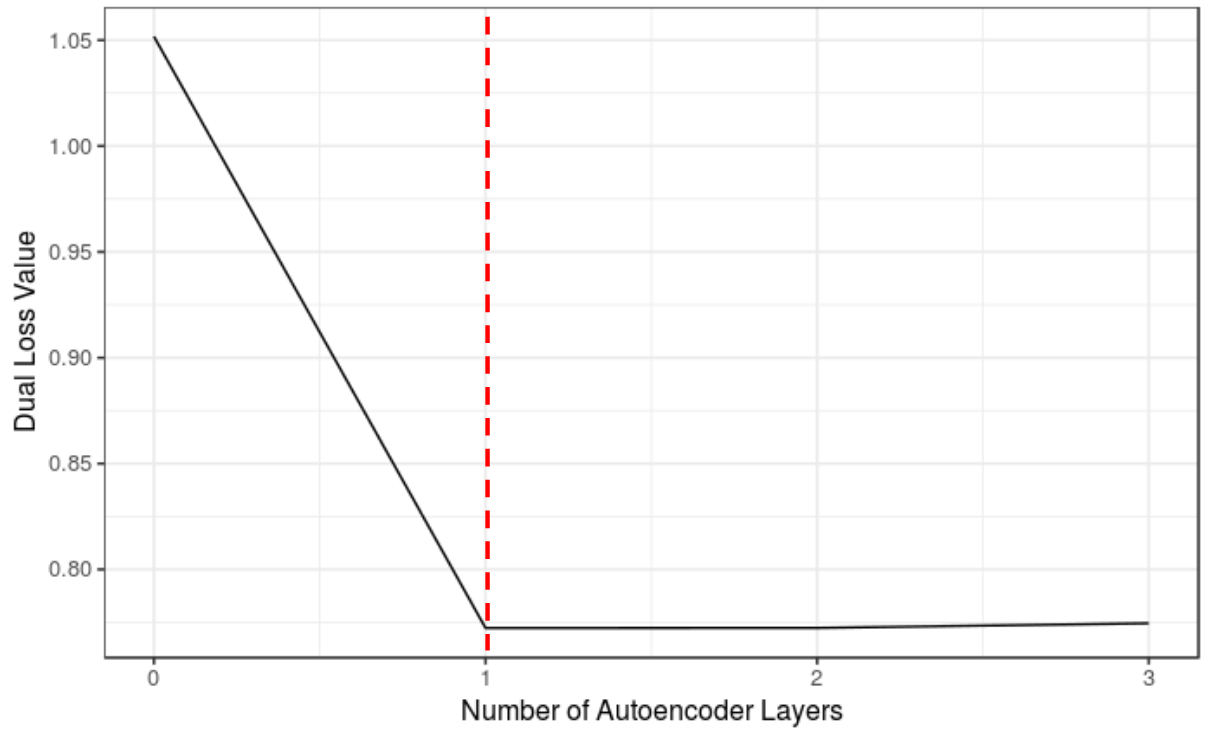
\includegraphics[width=\columnwidth]{figures/supplement/ae_layers.png}
	\caption{\textbf{Loss vs. Number of Autoencoder Layers}.
	After one hidden layer in both the encoder and the decoder, adding additional hidden layers to the autoencoder didn't have a large effect on how well Confounded performed.
	}
	\label{fig:ae}
\end{figure}

\paragraph{Adjust discriminator depth}

It is crucial that a batch adjuster be able to identify and model batch effects if it is to remove them.
This is particularly the case for Confounded, which tries to identify and remove even complex nonlinear batch and confounding effects.
The discriminator must be adequately powerful in order for the adversarial system to remove these effects.
A deeper discriminator, or one with more hidden layers, could potentially be more powerful in identifying these complex nonlinear relationships, but adding hidden layers to a network comes at the costs of longer training times and potentially less effective training. % Find a source for this.
Confounded's discriminator must then have a ``just right'' number of hidden layers to balance these benefits and costs.
Over testing the otherwise same architecture with different-depth discriminators, we found the general trend that as the number of hidden discriminator layers increases, the overall dual loss decreases (see \figurename{} \ref{fig:disc}).
There seemed to be a trough to this effect around 10 hidden layers, so we left 10 as the default.

\begin{figure}
	\centering
	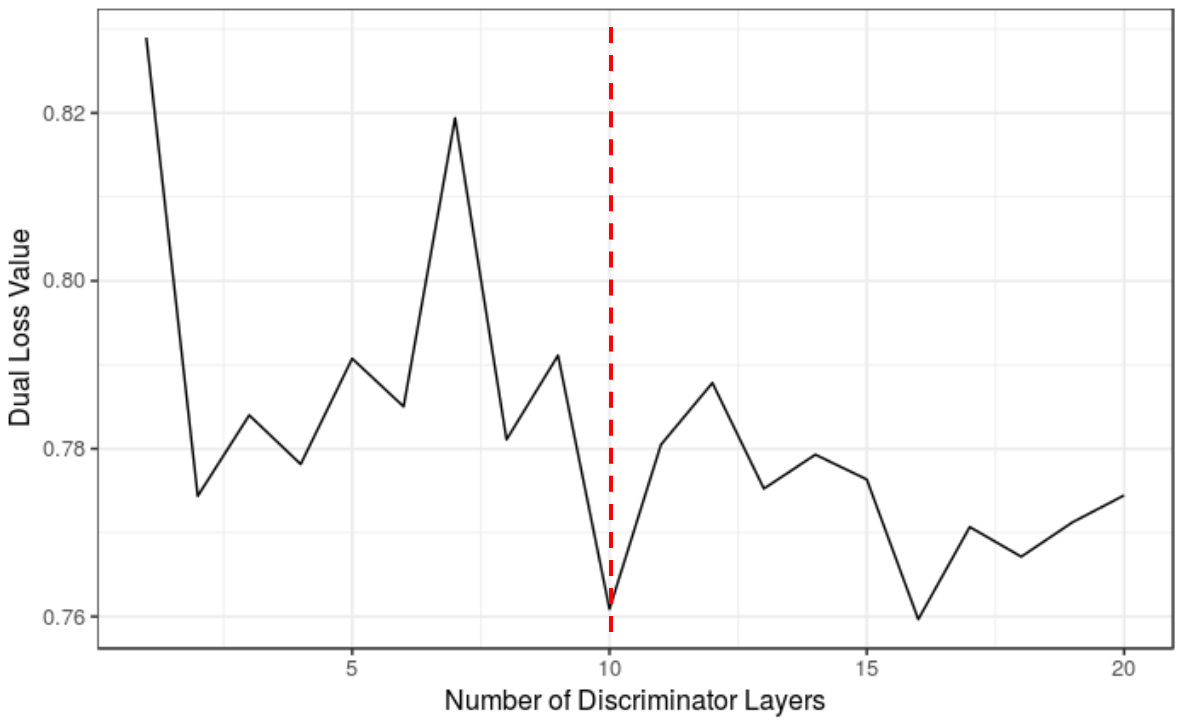
\includegraphics[width=\columnwidth]{figures/supplement/disc_layers.png}
	\caption{\textbf{Loss vs. Number of Discriminator Layers}.
	As the number of hidden layers increases in the discriminator, the dual loss generally decreases.
	This pattern happens naturally because the discriminator learns more slowly with more layers, but there seems to be a possible trough at 10 hidden layers.
	}
	\label{fig:disc}
\end{figure}

\paragraph{Scale to [0, 1] with sigmoid}

Neural networks typically perform better if their inputs are in the same range. % Find a source.
However, gene expression data often have highly variable column ranges. % Get the min and max for the TCGA dataset
Prior to passing data through Confounded, scaled each column to the same range, [0, 1].
Initially, we did this linearly by subtracting the minimum from each column and then dividing by the column range.
We then tried scaling the data using the sigmoid function, which scales values to [0, 1] but squishes very low or very high values more than the average values.
In both cases, we expand the data to the original range after adjustment by applying the inverse of the scaling function.
The sigmoid function appeared to give slightly better results (see \figurename{} \ref{fig:scaling}), so sigmoid scaling is Confounded's default.

\begin{figure}
	\centering
	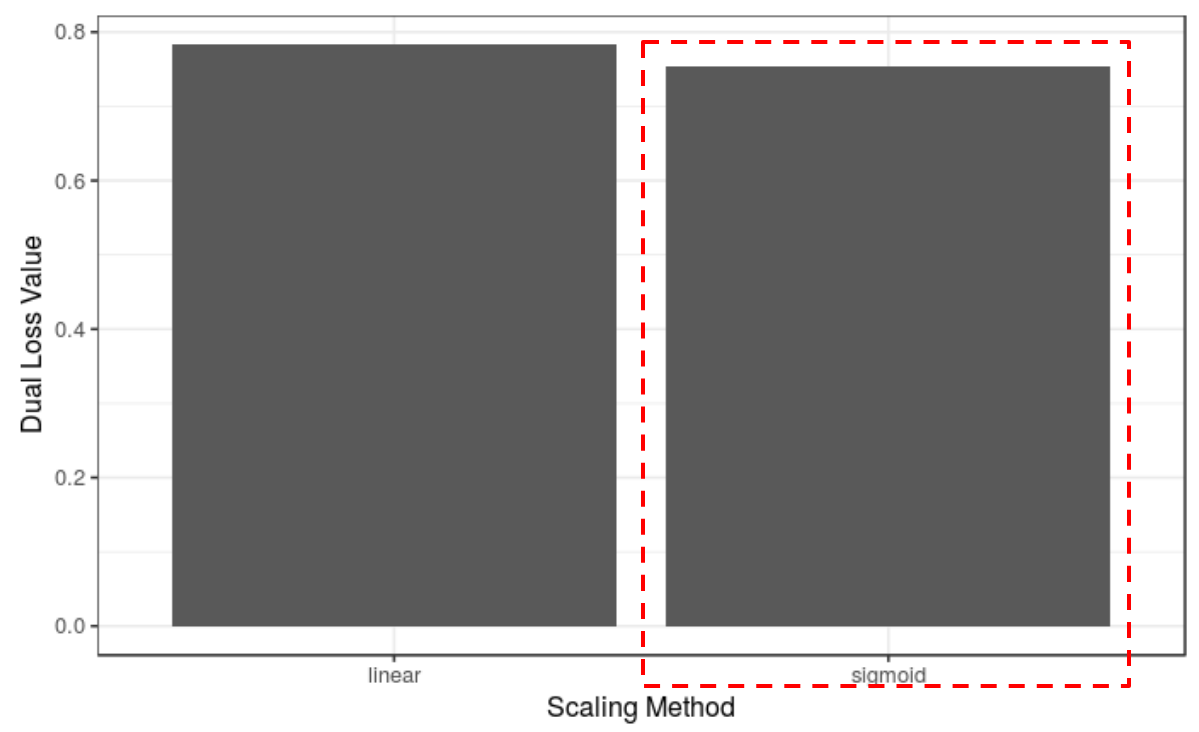
\includegraphics[width=\columnwidth]{figures/supplement/scaling.png}
	\caption{\textbf{Loss vs. Scaling Method}
	Confounded performed slightly better wen scaling the input data to [0, 1] with the sigmoid function rather than a linear scaling function.
	}
	\label{fig:scaling}
\end{figure}

\paragraph{Dropout in the discriminator}

When training initially with a plain autoencoder and discriminator (meaning subnetworks with only weights, biases, and activation functions), the network trained very poorly.
For example, the outputs for the MNIST datasets looked only like random noise rather than like handwritten digits.
We hypothesized that this may be because the discriminator was overfitting;
rather than learn what the batch effect looked like, it would memorize every sample in each batch, and then when it saw output from the autoencoder that looked like one of the memorized outputs, it would be able to predict the batch perfectly, regardless of whether the batch effect remained in the data.
In order to prevent this overfitting, we added dropout to all the layers with a probability of 50\%.
Once we added dropout, the network began to output images that looked like the original MNIST digits.
Our interpretation of this result is that dropout was able to successfully discourage the discriminator from overfitting.

\paragraph{Other unimplemented ideas}

We toyed with the idea of using convolutional layers \cite{krizhevsky_imagenet_2012-1} in the network because of their incredible success in the realm of image recognition.
We thought at first that a 20,000-dimensional vector of expression values was quite similar to a 200x100 image and that similar techniques could be used for both, which was encouraging because convolutional filters are quite efficient for processing images.
However, we were unable to devise a representation or arrangement of gene expression data points in which convolutional filters would make sense.
Although one could easily wrap a gene expression vector into two dimensions and arrange the genes by location in the genome, each data point fundamentally represents a completely different gene product.
Contrast this with image data, where each pixel represents the same data type (i.e. relative light intensities of some wavelength); if each pixel value was shifted to the left by one pixel, the image would still represent the same idea.
However, if each expression value were to be shifted one position to the left, it would in essence be like mistaking each gene product for another unrelated gene product.
Therefore, passing convolutional filters over a gene expression array, 1D or 2D, would not make sense since the relationship between a pair of consecutive genes is not necessarily analogous to the relationship between another pair of consecutive genes.
Because we couldn't justify any arrangement where spatial relationships between genes were consistently meaningful, we chose to only use fully connected layers in Confounded rather than convolutional layers.
We welcome any future intellectual advances that may allow convolutional networks and other image processing techniques to be applied to expression data.

The GSE37199 dataset has two levels of batches (``centre'' and ``plate'').
We identified this as an item of potential interest: can Confounded adjust for multiple batch levels of effects simultaneously?
However, we left this question for future research and chose instead to focus on the ``plate'' effect for this study.

\paragraph{Datasets}

Working with each new dataset enlightened us of a new edge case that hadn't yet been addressed in our code.
By applying to our methods to each of the four described datasets, our code became much more robust than if we had only developed and tested on one or two datasets.

\section{Data Format}

Confounded takes input data in the tidy data format \cite{wickham_tidy_2014-1}, namely:

\begin{itemize}
	\item Each row represents a different sample.
	\item Each column represents a different variable (either a clinical variable or a gene's expression).
\end{itemize}

Confounded parses through files in this format to determine which columns are discrete (integer or string) and which are continuous (floating point).
Each continuous column is interpreted to be a gene expression column and is adjusted for by the network according to the batch column.
This is one limitation to our software.
In a future iteration, it would be more robust to allow the user to specify continuous columns that should not be interpreted as gene expression data (e.g. ages in years with decimal precision representing fractions of years), or to pass expression values in as a different file or dataframe.
However for the datasets we tested, this didn't prove to be a problem.

\section{Testing different-sized datasets}

One big question that remained after testing our four datasets was why Confounded works better on some datasets and worse on others.
Our main hypothesis was that Confounded, like most tools that use deep learning, would inherently work better on larger datasets than on smaller ones.
We made two random subsets (sizes X and Y) of the TCGA dataset to assess how well Confounded performs relative to a scaling adjuster and to ComBat. % Put the actual sizes in here
Our results show that with the TCGA dataset, Confounded continues to outperform ComBat with the medium and smaller subsets (see \figurename{s} \ref{fig:mse}, \ref{fig:mmd}, \ref{fig:true_class}, and \ref{fig:batch}).
This may indicate that Confounded works better on more complex confounding effects, or perhaps that it works better with a smaller columnset (our TCGA dataset was restricted to 325 columns).
Future testing may be required to identify general cases when Confounded will outperform classic batch adjusters such as ComBat, but we anticipate that Confounded may be better particularly in removing confounding effects, whereas classic methods may be better on typical batch effects.

\newcommand{\disclaimer}{Note: the scaling function produced errors when run on the small TCGA dataset and was therefore not used in this chart.}

\begin{figure}
	\centering
	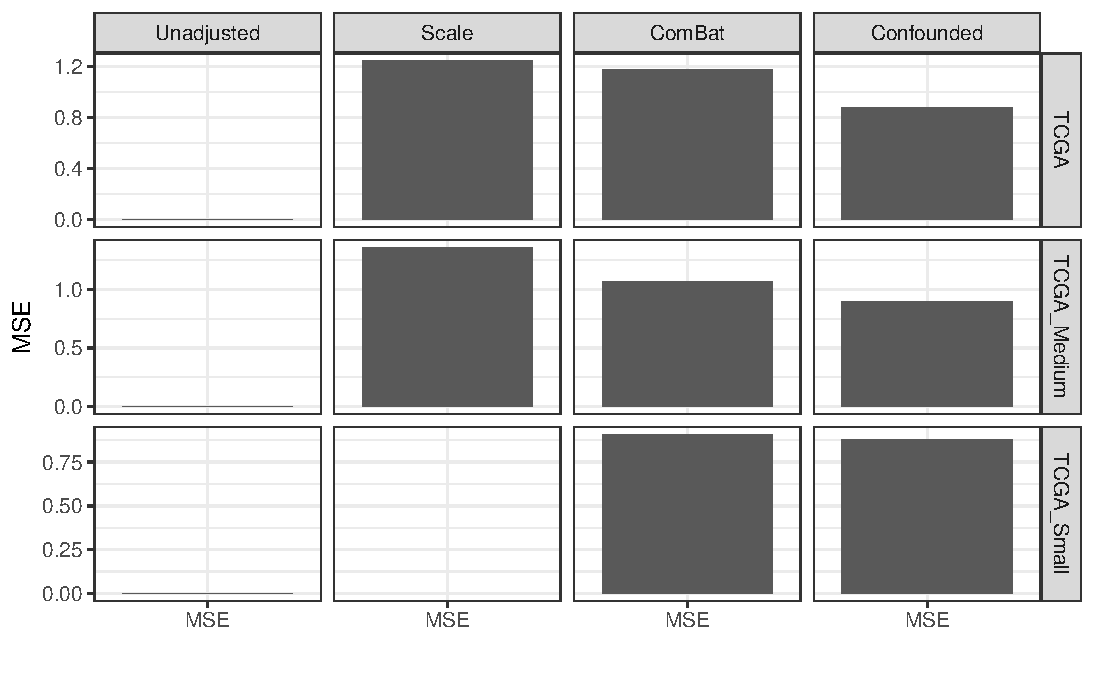
\includegraphics[width=\columnwidth]{figures/supplement/tcga_mse.pdf}
	\caption{\textbf{TCGA MSE}.
	Confounded consistently outperforms other adjusters with different sizes of the TCGA dataset in terms of mean squared error, meaning that Confounded is less disruptive to the original data.
	\disclaimer{}
	}
	\label{fig:mse}
\end{figure}
\begin{figure}
	\centering
	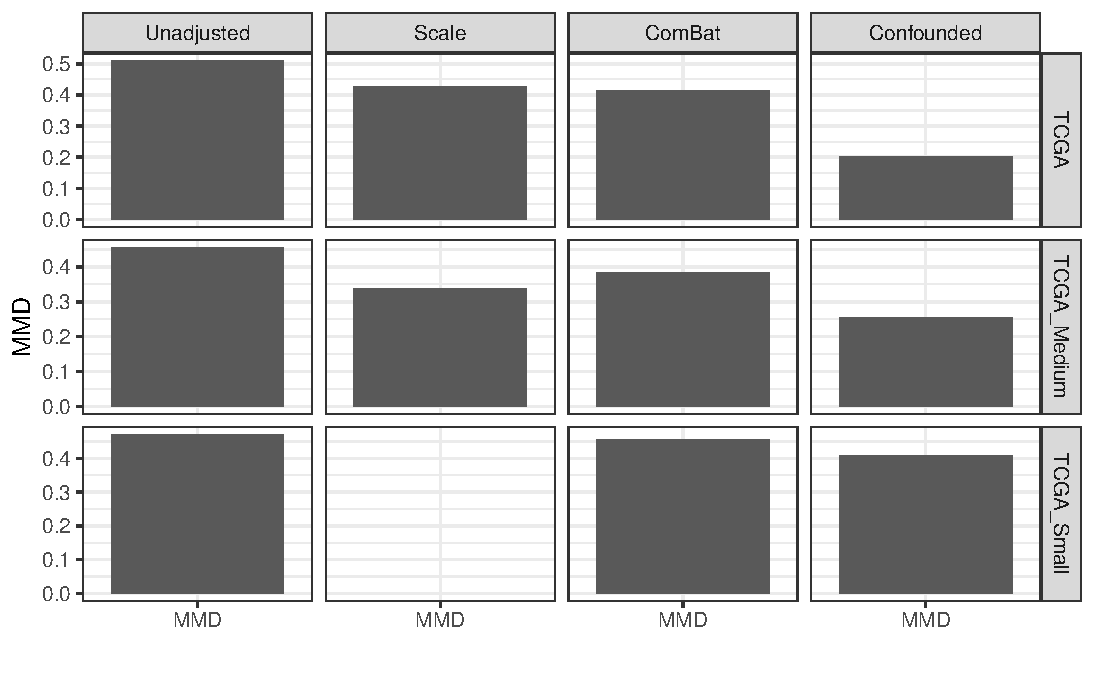
\includegraphics[width=\columnwidth]{figures/supplement/tcga_mmd.pdf}
	\caption{\textbf{TCGA MMD}
	Confounded outperforms other adjusters on the different sizes of the TCGA dataset in terms of max mean discrepancy, meaning that Confounded better aligns the expression value distributions between different cancer types.
	\disclaimer{}
	}
	\label{fig:mmd}
\end{figure}
\begin{figure}
	\centering
	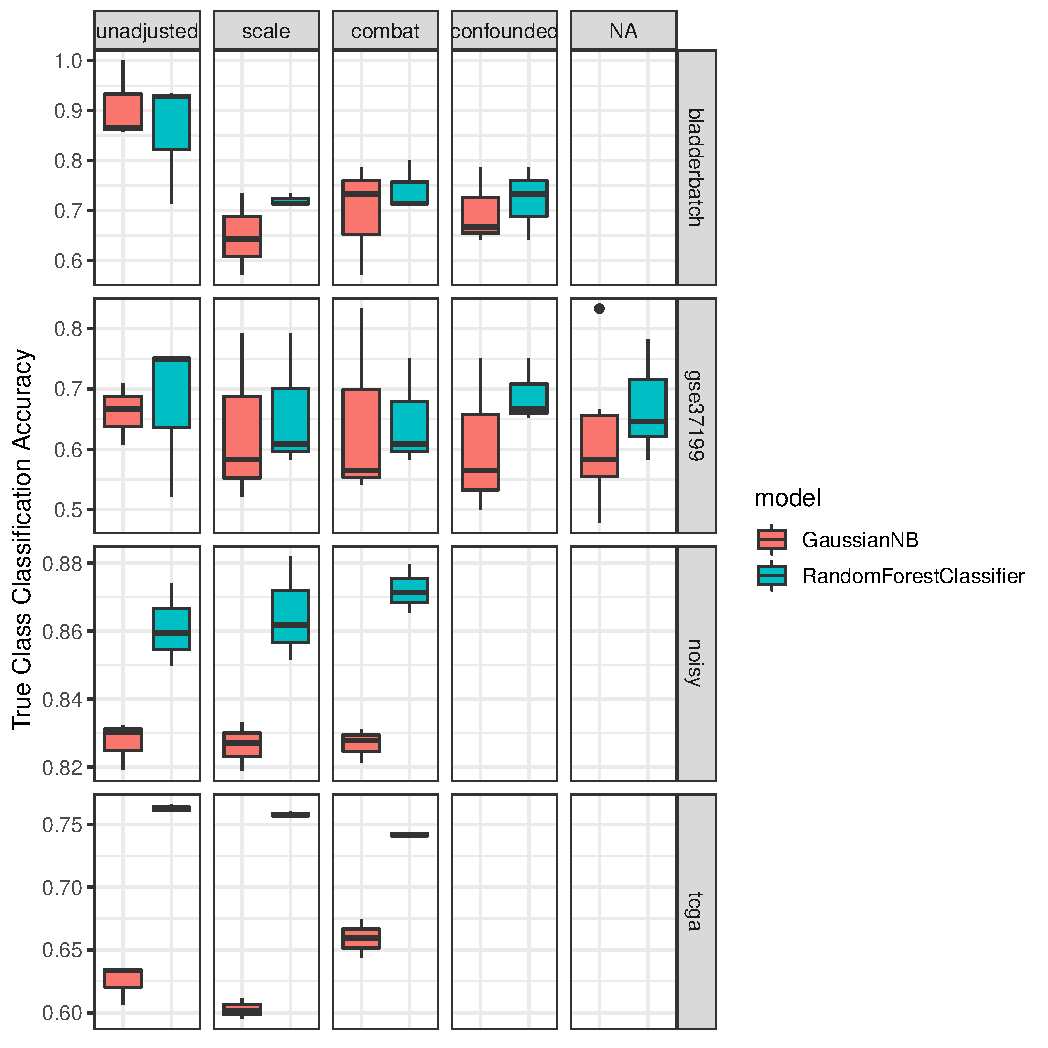
\includegraphics[width=\columnwidth]{figures/supplement/tcga_true_class_accuracy.pdf}
	\caption{\textbf{TCGA True Class Accuracy}.
	Confounded typically has a lower true class accuracy than the other adjusters for the TCGA dataset.
	However, this is likely because the true class (TP53 mutation status) is confounded with the batch (CancerType) that we've tried to remove.
	\disclaimer{}
	}
	\label{fig:true_class}
\end{figure}
\begin{figure}
	\centering
	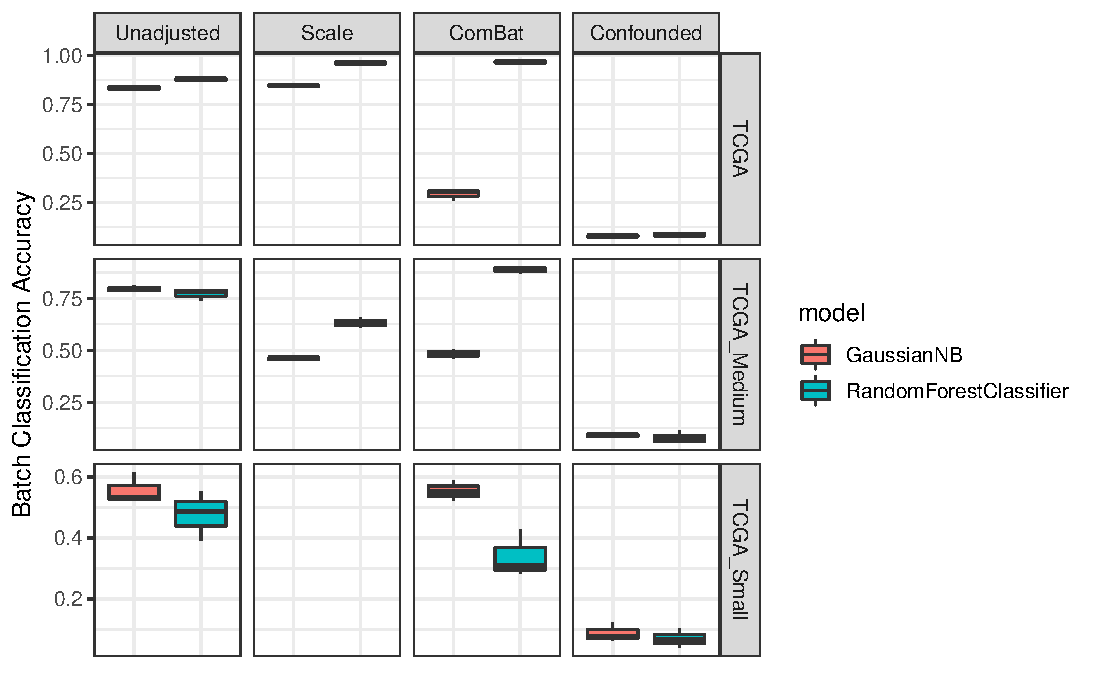
\includegraphics[width=\columnwidth]{figures/supplement/tcga_batch_accuracy.pdf}
	Confounded consistently removes more of the batch effects than the other adjusters as measured by Naive Bayes and Random Forests classification accuracy.
	\caption{\textbf{TCGA Batch Accuracy}
	\disclaimer{}
	}
	\label{fig:batch}
\end{figure}

\section{Other methods}

We wanted to also compare with SVA \cite{leek_capturing_2007} and the work of \citet{shaham_removal_2017} \citep{shaham_removal_2017,shaham_batch_2018} but were unable to get these two methods running.
With SVA, the documentation showed how to identify surrogate variables and use them in modeling, but we were unable to find examples of removing the effects that those surrogate variables represent.
We were unable to get \citet{shaham_removal_2017}'s methods running on our datasets, and we believe that this is due to some underlying assumptions that make their code more applicable to larger datasets.

\section{Metrics used}

\paragraph{MSE}

We calculate MSE by the following:

\begin{equation}
	\label{mse}
	MSE = \frac{1}{n}\sum_{i=1}^n{(\hat{x}_i - x_i)^2}
\end{equation}

Where $x$ represents the values in the autoencoder's input and $\hat{x}$ represents the approximated values in the output.
If $x = \hat{x}$, MSE will be 0.

\paragraph{MMD}

We calculated MMD using the following formula:

\begin{equation}
	\label{mmd}
	MMD(x, y) = \frac{1}{n^2}\sum_{i=1}^n{\sum_{j=1}^n{k(x_i, x_j)}} - \frac{2}{nm}\sum_{i=1}^n{\sum_{j=1}^m{k(x_i, y_j)}} + \frac{1}{m^2}\sum_{i=1}^m{\sum_{j=1}^m{k(y_i, y_j)}}
\end{equation}

Where $k(x, y)$ is the Gaussian kernel between $x$ and $y$ as implemented in \texttt{sklearn.metrics.pairwise.rbf\_kernel}, and where $x$ represents the data from one batch and $y$ represents the data from another batch.
In cases where there were more than two batches (e.g. $x$, $y$, and $z$), we averaged the pairwise MMD values to calculate an overall MMD.

\paragraph{MNIST PCA \& t-SNE}

See \figurename{s} \ref{fig:pca} and \ref{fig:tsne}.

\begin{figure}
	\centering
	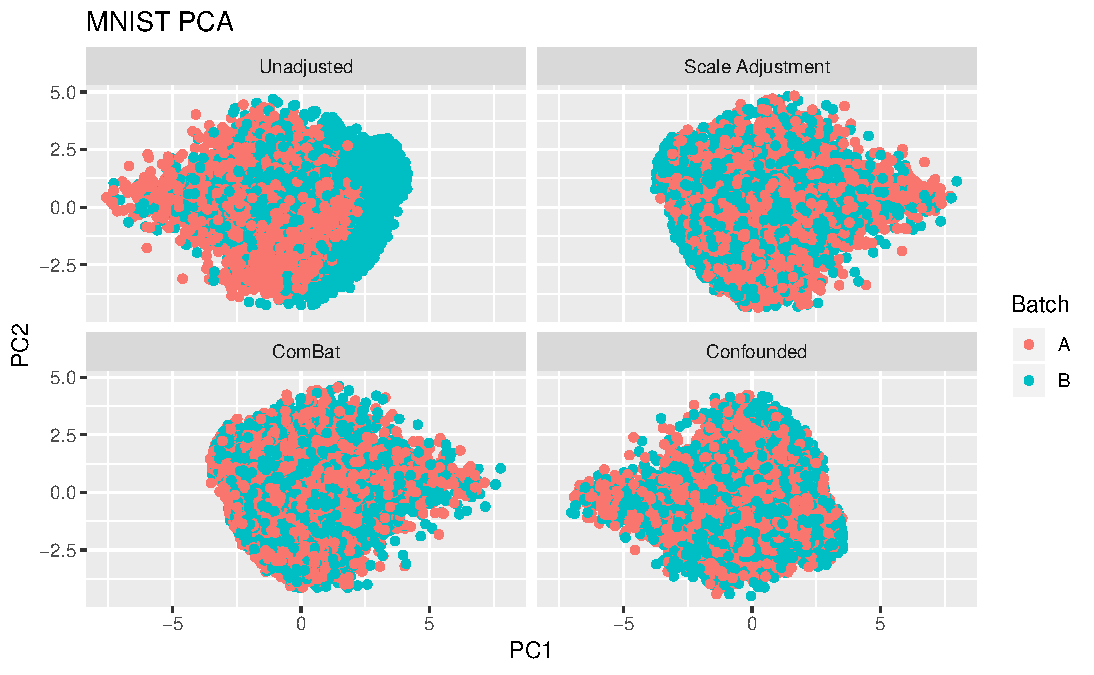
\includegraphics[width=\columnwidth]{figures/supplement/mnist_pca.pdf}
	\caption{\textbf{MNIST PCA}
	All adjusters seem to remove the strong linear batch effect in the MNIST dataset.
	}
	\label{fig:pca}
\end{figure}
\begin{figure}
	\centering
	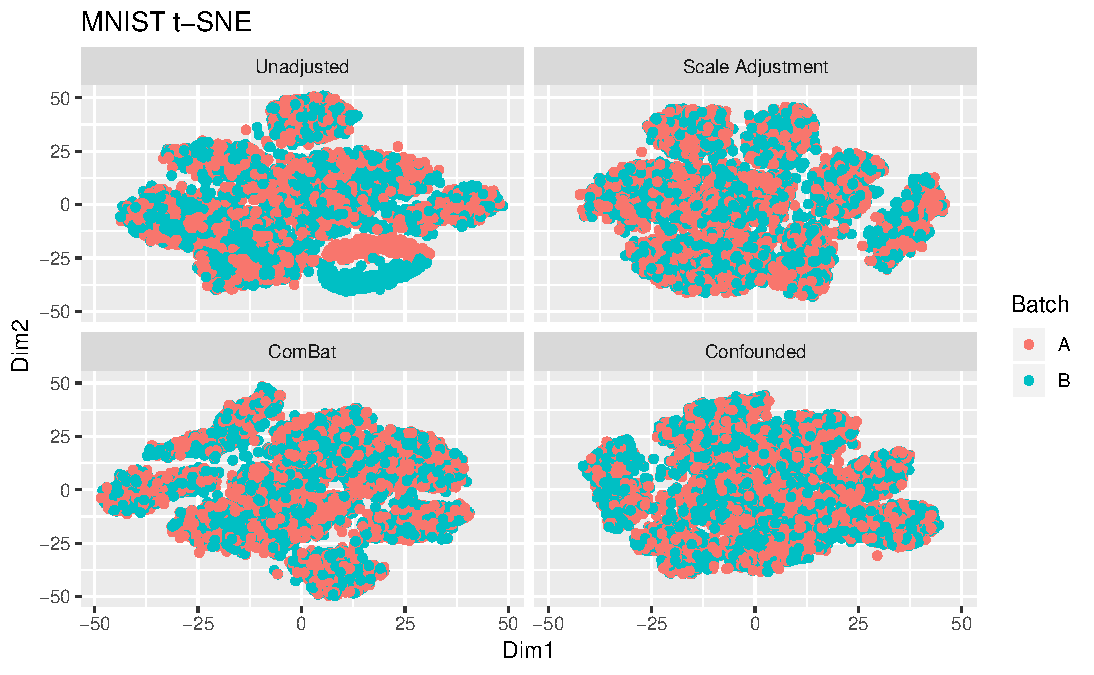
\includegraphics[width=\columnwidth]{figures/supplement/mnist_tsne.pdf}
	\caption{\textbf{MNIST t-SNE}
	Both ComBat and Confounded seem to remove batch effect from the MNIST dataset as shown by a t-SNE plot.
	}
	\label{fig:tsne}
\end{figure}

\bibliography{references}

\end{document}
